\chapter{Revisão bibliográfica}\label{cap:revisao}

Esta seção apresenta conceitos e fundamentos teóricos para o desenvolvimento deste trabalho. São apresentados tópicos relacionados a comunicação por satélites, evolução do sistema ARGOS, e técnicas de modulação, codificação e sincronização envolvidas no padrão \gls{PTT-A3}. O objetivo é fornecer uma base de conhecimento para a compreensão dos requisitos técnicos e operacionais do sistema de comunicação proposto.

\section{COLETA DE DADOS SBCDA VIA SATÉLITE }\label{sec:sbcda}

A comunicação por satélites desempenha um papel fundamental na coleta e disseminação de dados ambientais em escala regional e global. No contexto brasileiro, essa função é desempenhada pelo \gls{SBCDA}, operado pelo \gls{INPE}. O \gls{SBCDA} é composto pelos satélites \gls{SCD-1}, \gls{SCD-2} e \gls{CBERS-1} até \gls{CBERS-4} apresentados na \autoref{fig:satelites} abaixo, que orbitam a aproximadamente 750 km de altitude, recebendo informações transmitidas por \gls{PCD} espalhadas pelo território nacional \cite{lima_parallel_2021}.


\begin{figure}[ht]
    \centering
    \caption{Satélites para coleta de dados ambientais}
    \label{fig:satelites}
    \begin{minipage}[t]{0.48\linewidth}
      \centering
      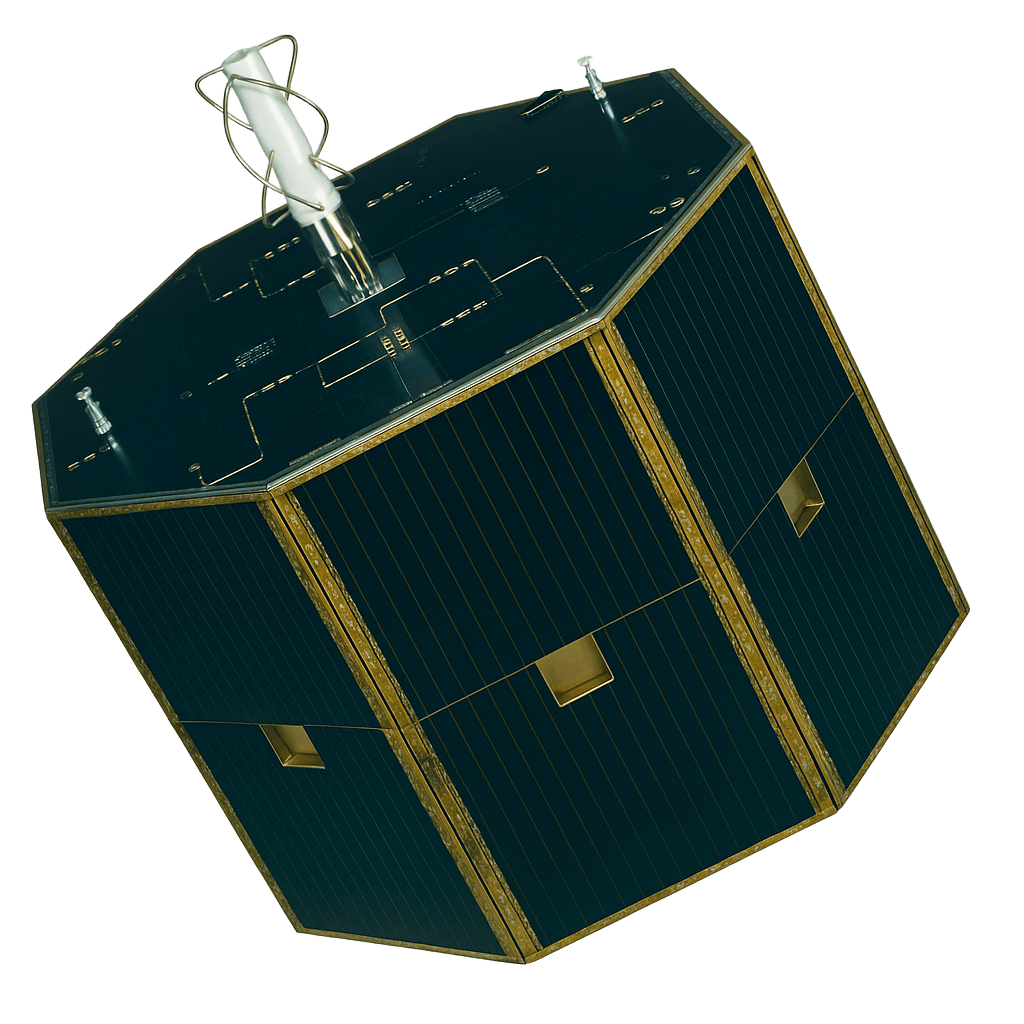
\includegraphics[width=0.7\linewidth]{assets/sat-SCD-1.png}
      \vspace{0.5em}
      \caption*{Satélite SCD-1}
      \small
      \begin{tabularx}{\linewidth}{>{\centering\arraybackslash}X >{\centering\arraybackslash}X}
        \toprule
        \textbf{Parâmetro} & \textbf{Valor} \\
        \midrule
        Massa & 115 kg \\
        Potência Elétrica & 110 W \\
        Vida útil & 4 anos \\
        Altitude média & $\approx$ 750 km \\
        Inclinação orbital & 25$^\circ$ \\
        Período orbital & 99,7 min \\
        \bottomrule
      \end{tabularx}
    \end{minipage}
    \hfill
    \begin{minipage}[t]{0.48\linewidth}
      \centering
      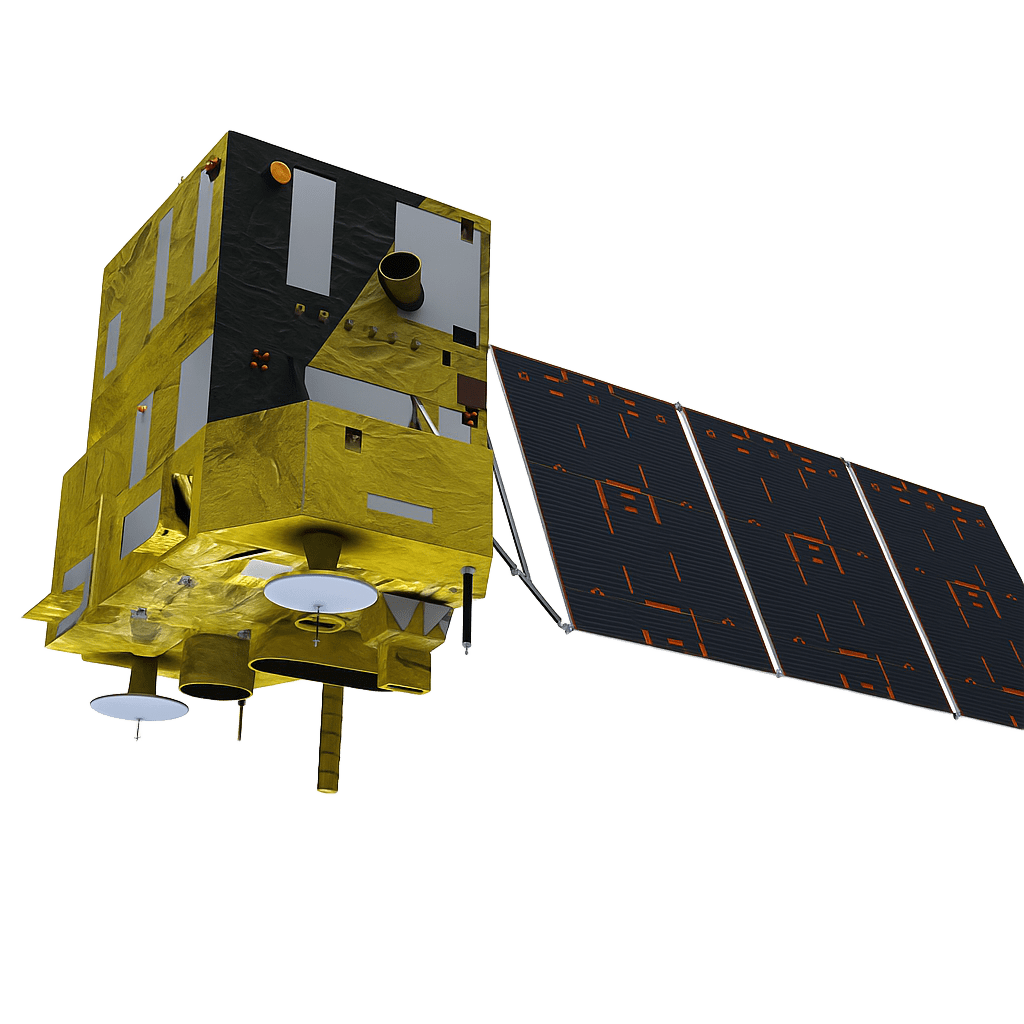
\includegraphics[width=0.7\linewidth]{assets/sat-CBERS-4.png}
      \vspace{0.5em}
      \caption*{Satélite CBERS-4}
      \small
      \begin{tabularx}{\linewidth}{>{\centering\arraybackslash}X >{\centering\arraybackslash}X}
        \toprule
        \textbf{Parâmetro} & \textbf{Valor} \\
        \midrule
        Massa & 1 980 kg \\
        Potência Elétrica & 2 300 W \\
        Vida útil & 3 anos \\
        Altitude média & $\approx$ 778 km \\
        Inclinação orbital & 98,54$^\circ$ \\
        Período orbital & 100,32 min \\
        \bottomrule
      \end{tabularx}
    \end{minipage}
    \vspace{0.5em}
    
\end{figure}

Esses satélites recebem sinais transmitidos pelas \gls{PCD} na faixa de frequência UHF (401,62 a 401,65 \gls{mhz}) e os retransmitem para as \gls{ETR} localizadas em solo, nas faixas de Banda-S (2267,5 \gls{mhz}). Como operam em órbitas baixas, esses satélites realizam aproximadamente 14 revoluções por dia sobre o território nacional, o que permite ampla cobertura espacial.

Apesar da ampla cobertura, a comunicação com satélites de órbita baixa apresenta um grande desafio técnico, sendo a necessidade de visada simultânea entre a \gls{PCD} transmissora e o satélite, o que limita a janela de transmissão e impõe restrições na coleta contínua de dados. Além disso, o movimento relativo entre a \gls{PCD} e o satélite provoca o chamado efeito Doppler, responsável por deslocamentos na frequência do sinal recebido, podendo atingir até ±79,4 kHz. Esse desvio precisa ser compensado para garantir a correta demodulação do sinal \cite{rae2005detector, rodrigues_demodulador_2018}.

A confiabilidade do enlace também é impactada por fatores como atenuação no espaço livre, ruídos térmicos, e variações atmosféricas. Para compensar esses fatores, são necessárias técnicas específicas de modulação, sincronização, codificação de dados e planejamento de enlace, de modo a garantir a confiabilidade das mensagens transmitidas.

\subsection{Constelação Catarina}

A Constelação Catarina é um projeto nacional baseado no uso de nanossatélites em órbita baixa, para atuar como um novo braço operacional do \gls{SBCDA}. A Constelação Catarina é composta por pequenos satélites integrados com \gls{SDR}, capazes de receber sinais transmitidos pelas \gls{PCD} no padrão \gls{ARGOS-II}, com planos futuros de migração para o padrão \gls{ARGOS-III} \cite{gomes_otimizacao_2024}.

Diferentemente dos satélites tradicionais, os nanosatélites da Constelação Catarina são projetados para realizar a decodificação e o armazenamento dos dados a bordo, o que permite superar a limitação de visada simultânea entre satélite e \gls{ETR}, ampliando a cobertura do sistema \cite{rodrigues_demodulador_2018}.

A arquitetura dos satélites que compõem a constelação é baseada na integração do transceptor \gls{AD9361} com uma \gls{FPGA} da \gls{Zynq-7000}, formando uma plataforma de \gls{SDR} altamente flexível \footnote{https://www.argos-system.org/wp-content/uploads/2023/01/ARTIC-Chipset-AnSem-Info-sheet.pdf}. Essa configuração permite a reconfiguração remota do hardware, o que é especialmente importante para futuras atualizações de protocolo ou migração para novos padrões de comunicação, como o \gls{PTT-A3}.


\section{EVOLUÇÃO DO SISTEMA ARGOS}\label{sec:quadros}

O \gls{ARGOS-II}, base do \gls{SBCDA} desde 1993, utiliza transmissores do tipo \gls{PTT-A2}, baseados em modulação analógica \gls{PM} com codificação Manchester. Essa versão se mostrou eficiente por muitos anos, mas suas limitações logo se tornaram evidentes, especialmente no que diz respeito à robustez frente a ruído, à largura de banda ocupada e à necessidade de visada simultânea entre \gls{PCD} e satélite para a \gls{ETR} \cite{cnes_services_and_message_formats_ed2_rev2_2006}.

A evolução desse sistema levou ao desenvolvimento do \gls{ARGOS-III}, que introduziu novas técnicas digitais de comunicação. Essa nova geração incorporou transmissores do tipo \gls{PTT-A3} e \gls{PTT-ZE}, os quais se destacam pela adoção de modulação \gls{QPSK}, codificação convolucional e embaralhamento de dados, resultando em maior confiabilidade na transmissão e maior eficiência espectral. Além disso, o \gls{ARGOS-III} permite o armazenamento e retransmissão de mensagens a bordo do satélite para a \gls{ETR} \cite{lima_parallel_2021, rodrigues_demodulador_2018}.

\section{ESPECIFICAÇÕES DO PADRÃO PTT-A3}

O transmissor do tipo \gls{PTT-A3} é um dos formatos definidos na terceira geração do sistema \gls{ARGOS}, projetado para oferecer maior robustez na transmissão e maior eficiência na utilização do espectro de frequência. 

A estrutura de um quadro \gls{PTT-A3} é composta por três campos principais, sendo eles: portadora pura, palavra de sincronismo (preâmbulo) e datagrama. Na \autoref{fig:estrutura_quadro}, a estrutura é apresentada de forma detalhada, considerando que a taxa de transmissão \gls{Rb} é de 400 \gls{bps} \textcite{cnes_services_and_message_formats_ed2_rev2_2006}.

\begin{figure}[ht]
	\centering
	\caption{Estrutura do quadro de transmissão ARGOS-3}\label{fig:estrutura_quadro}
	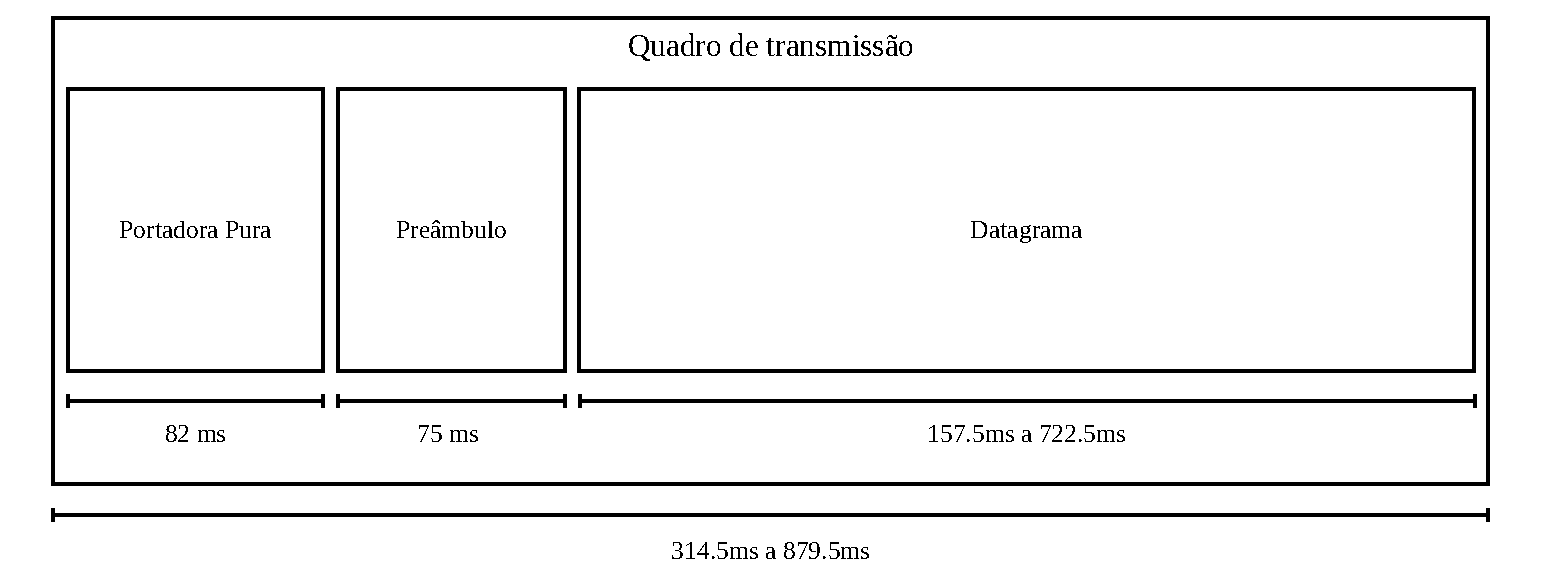
\includegraphics[width=\linewidth]{assets/quadro.pdf}
\end{figure}

\subsection{Portadora pura}

A sequência de transmissão do quadro inicia-se com a portadora contínua ou pura, com duração de 82 ± 2 ms. Durante essa etapa a portadora não transmite dados modulados e é utilizada pelo receptor apenas para realizar a detecção do sinal, bem como para facilitar o processo de sincronização de frequência e fase da portadora. 

A \autoref{fig:portadora_pura_freq} apresenta o sinal da portadora pura no espectro em comparação com o sinal modulado. Nota-se que quando apenas a portadora pura é transmitida, o espectro do sinal é concentrado em uma única frequência, sem componentes laterais. Já o sinal modulado apresenta componentes laterais que se estendem ao redor da frequência da portadora \gls{fc}, formando uma banda de uso do espectro mais ampla \cite{cnes_services_and_message_formats_ed2_rev2_2006}.


\begin{figure}[ht]
	\centering
	\caption{Simulação de portadora pura no domínio da frequência}\label{fig:portadora_pura_freq}
	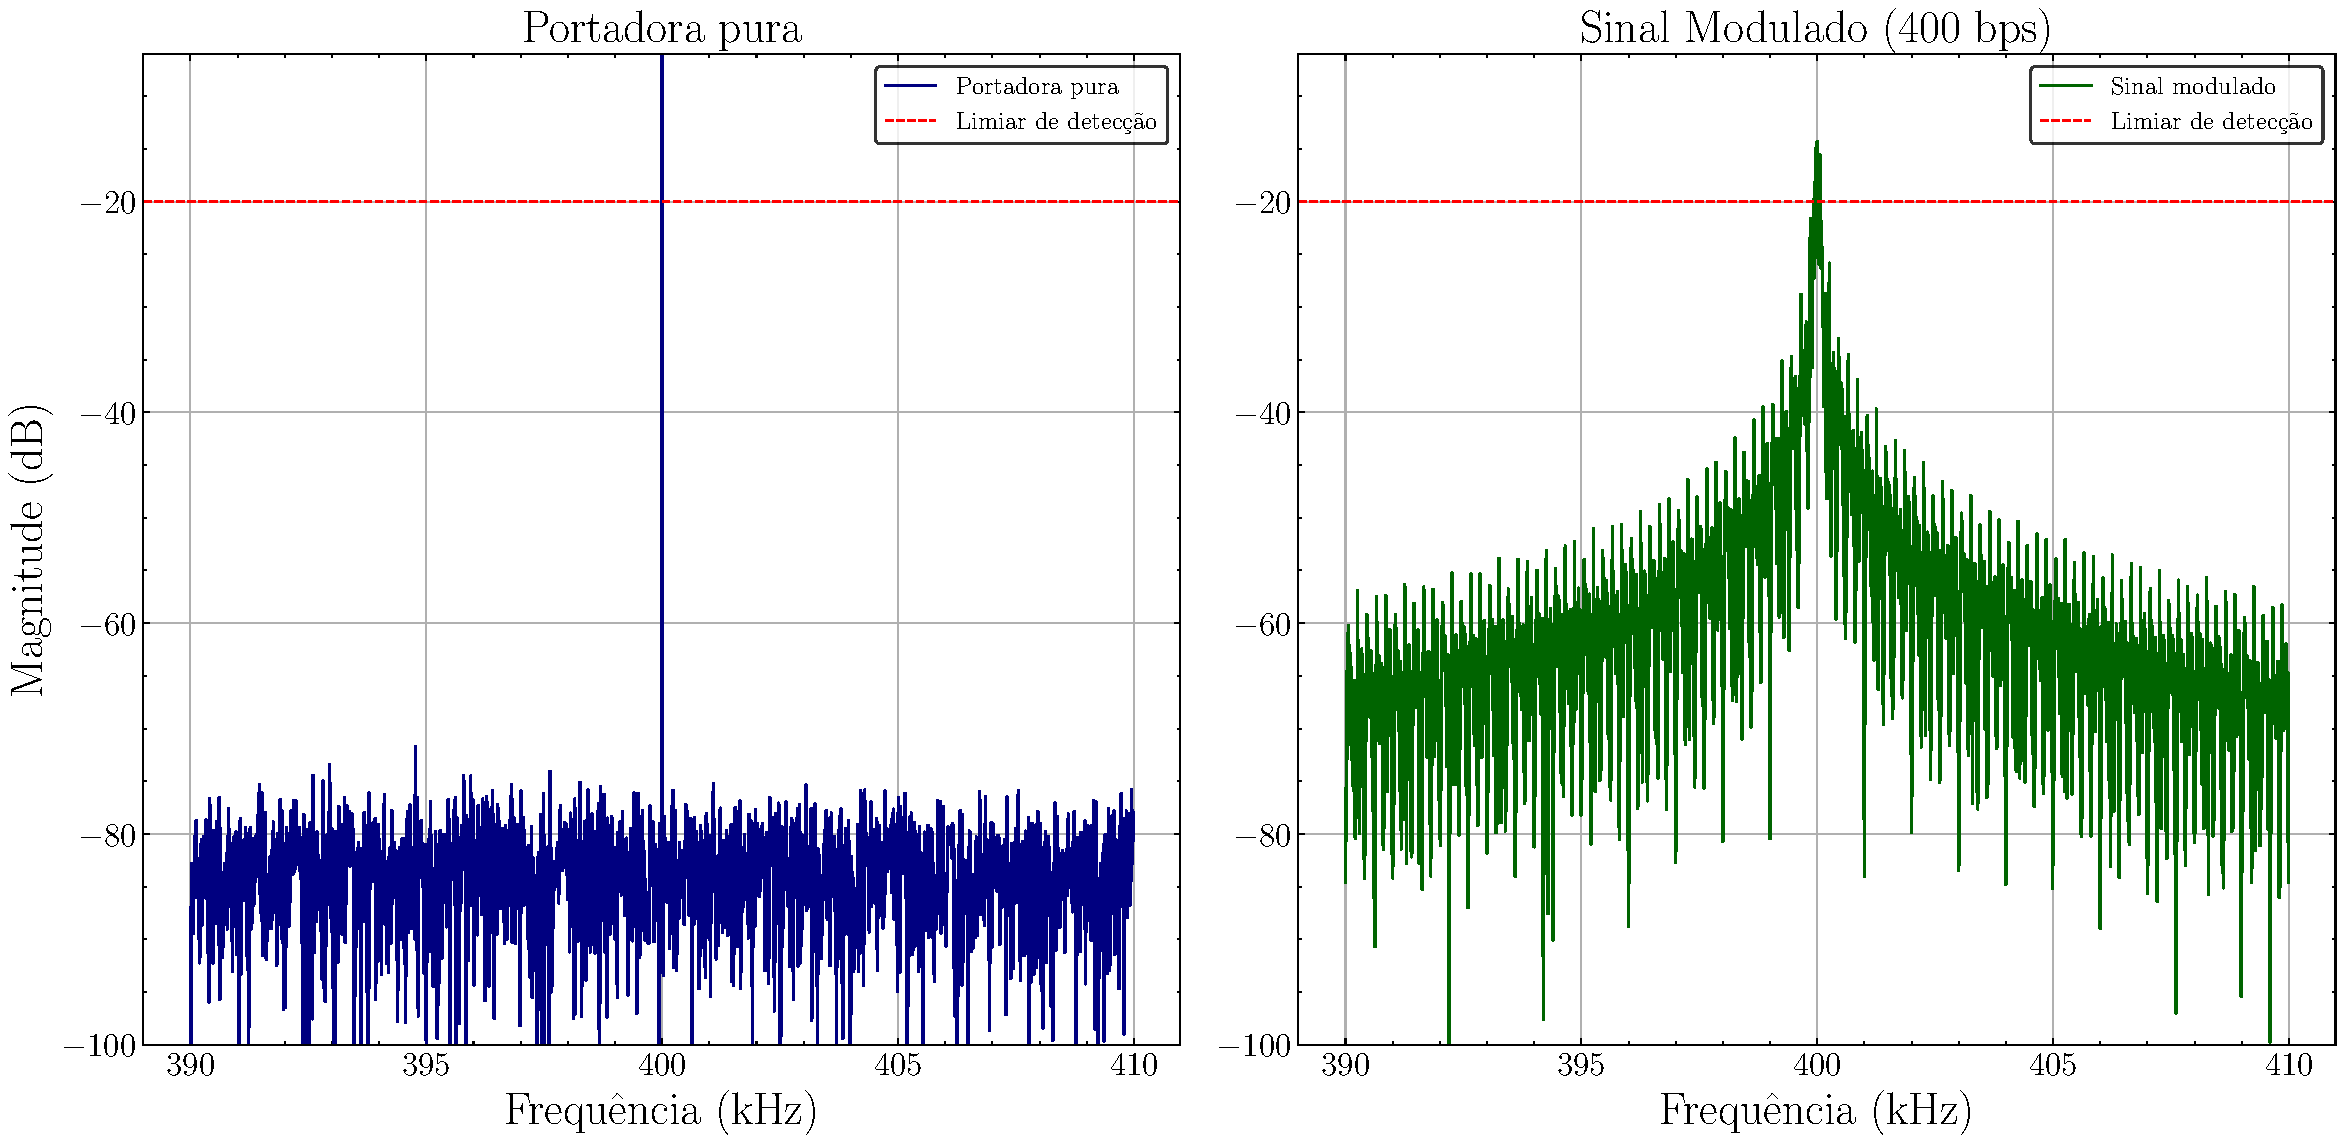
\includegraphics[width=\linewidth]{assets/plots/carrier_spectra.pdf}
    
\end{figure}

O processo de detecção do sinal realizado pelo receptor monitora a presença de sinal que ultrapassa um determinado limiar, dessa forma é fundamental que no receptor o sinal esteja o mais concentrado e com a maior \gls{SNR} possível no momento da detecção, para que a frequência da portadora, \gls{fc}, seja identificada corretamente \cite{cnes_services_and_message_formats_ed2_rev2_2006}.


\subsection{Palavra de sincronismo}

Logo após a portadora pura, é transmitida uma palavra de sincronismo de 30 bits (correspondente a 15 símbolos \gls{QPSK}), cuja função é auxiliar na identificação do início da mensagem codificada, possibilitando a sincronização para decisão. Essa sequência é conhecida e fixa entre transmissor e receptor, no caso do \gls{PTT-A3} sendo $S = \text{2BEEEEBF}_{16}$, o que permite alinhar corretamente a decisão e identificar o início do bloco de dados úteis. \cite{cnes_services_and_message_formats_ed2_rev2_2006}

A sequência \gls{Sn} é separada em dois vetores distintos, \gls{SIn} e \gls{SQn}, por meio de uma intercalação simples de seus bits. O processo de intercalação consiste em distribuir os bits de forma alternada entre os canais \gls{SIn} e \gls{SQn}, resultando em duas sequências de 15 bits cada, que serão transmitida como preâmbulo \cite{cnes_services_and_message_formats_ed2_rev2_2006}, usando a sequência padrão do \gls{ARGOS-III} podemos representar como

\vspace{-1em}
\begin{equation}
\begin{aligned}
    S_I[n] &= [S_0,\ S_2,\ S_4,\ \dots,\ S_{28}] &\mapsto&  S_I[n] = [1111,\ 1111,\ 1111,\ 111]     \\
    S_Q[n] &= [S_1,\ S_3,\ S_5,\ \dots,\ S_{29}] &\mapsto&  S_Q[n] = [0011,\ 0101,\ 0100,\ 111]
\end{aligned}
\label{eq:intercalacao}
\end{equation}

\noindent Importante destacar que esta palavra não é codificada convolucionalmente ou embaralhada, sendo adicionada ao início do vetor de bits de cada canal após esses blocos.  \cite{cnes_services_and_message_formats_ed2_rev2_2006}. 

\subsection{Datagrama}

Após o envio da palavra de sincronismo, inicia-se a transmissão dos dados modulados. Esses dados são organizados segundo a estrutura definida pelo datagrama do padrão \gls{ARGOS-III}, que contém os campos responsáveis pela identificação da plataforma, carga útil de dados e controle de finalização, conforme apresentado na \autoref{fig:datagrama} \cite{cnes_services_and_message_formats_ed2_rev2_2006}.

\begin{figure}[ht]
	\centering
	\caption{Estrutura do datagrama ARGOS-3}\label{fig:datagrama}
	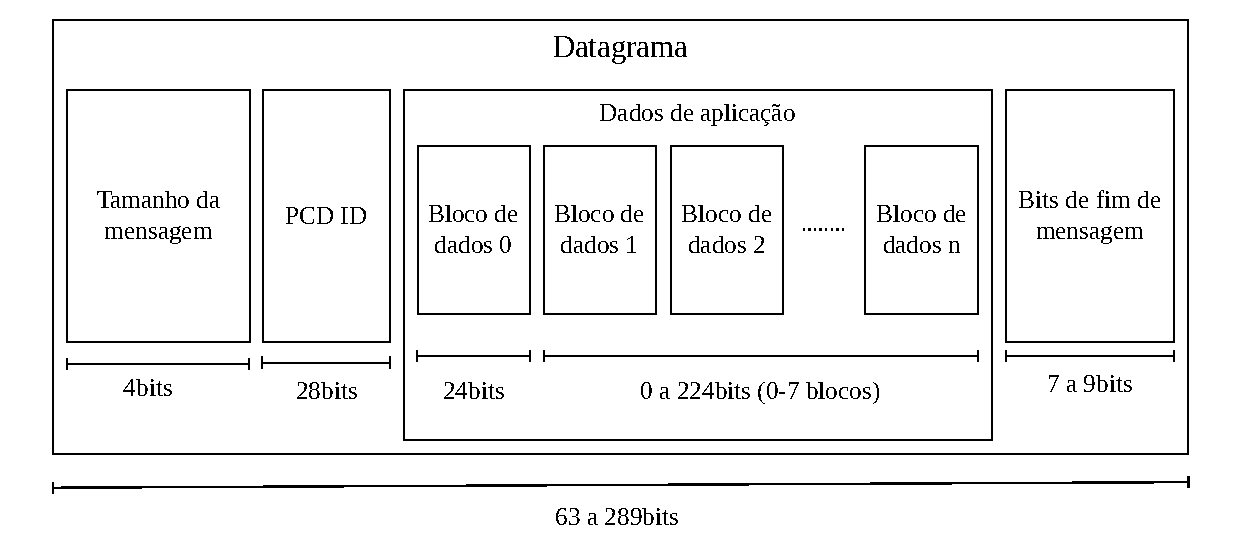
\includegraphics[width=\linewidth]{assets/datagrama.pdf}
    
\end{figure}

\section{ESTRUTURA DE UM DATAGRAMA ARGOS-3}

O datagrama transmitido no padrão \gls{ARGOS-III} possui uma estrutura bem definida, composta por campos de dados do usuário, que carregam as informações provenientes dos sensores da \gls{PCD}, e por campos de cabeçalho, responsáveis por identificar a estação transmissora e informar o comprimento total da mensagem. Esses campos incluem o identificador da PCD, o número de blocos de dados e um bit de paridade, que auxilia na verificação de integridade da informação. Essa organização permite que o sistema receptor interprete corretamente o conteúdo transmitido e associe os dados recebidos à plataforma correspondente.


\subsection{Dados de aplicação}

A primeira etapa na montagem do datagrama consiste na coleta dos dados de aplicação, isto é, os dados que efetivamente contêm informação dos sensores a serem transmitidos da \gls{PCD} para o satélite.

\subsubsection{Sensores}

Cada sensor presente nas \gls{PCD} gera um valor de oito bits correspondente à variável monitorada, possibilitando assim 256 ($2^8$) níveis de monitoramento para cada sensor. A PCD pode ser equipada com diferentes sensores, de acordo com o cenário de instalação e os parâmetros ambientais de interesse. 

Entre os sensores comumente utilizados, destacam-se os de direção do vento ($^{\circ}$), precipitação (mm), pressão atmosférica (mB), radiação solar acumulada (MJ/m2), temperatura do ar ($^{\circ}\text{C}$), umidade relativa ($\%$), e velocidade do vento (m/s). Por exemplo, os dados \footnote{http://sinda.crn.inpe.br/PCD/SITE/novo/site/historico/action.php} coletados da PCD 31855 são mostrados no \autoref{quadro:dados-meteorologicos}.


\begin{quadro}[ht]
\caption{Dados meteorológicos da PCD 31855 (10/10/2007 - 11/10/2007)}\label{quadro:dados-meteorologicos}
\resizebox{\textwidth}{!}{%
\begin{tabular}{lccccccc}
    \toprule
    \textbf{DataHora} & \textbf{DirVento} & \textbf{Precip.} & \textbf{PressãoAtm} & \textbf{RadSolAcum} & \textbf{TempAr} & \textbf{UmidRel} & \textbf{VelVento} \\
    \midrule
    2007-11-10 21h & 0 & 0 & 945.5 & 2.3  & 30.8 & 25.6 & 0 \\
    2007-11-10 18h & 0 & 0 & 943.8 & 8.75 & 36.5 & 20.8 & 0 \\
    2007-11-10 15h & 0 & 0 & 947.3 & 9.72 & 33.6 & 28.8 & 0 \\
    2007-11-10 12h & 0 & 0 & 950.1 & 4.98 & 28.0 & 51.2 & 0 \\
    2007-11-10 09h & 0 & 0 & 949.3 & 0.17 & 20.9 & 60.8 & 0 \\
    2007-11-10 06h & 0 & 0 & 947.8 & 0.00 & 21.8 & 52.8 & 0 \\
    2007-11-10 03h & 0 & 0 & 948.0 & 0.00 & 23.5 & 40.0 & 0 \\
    2007-11-10 00h & 0 & 0 & 948.4 & 0.00 & 21.9 & 35.2 & 0 \\
    2007-11-09 21h & 0 & 0 & 946.1 & 0.48 & 30.8 & 20.8 & 0 \\
    2007-11-09 18h & 0 & 0 & 945.1 & 9.13 & 36.3 & 16.0 & 0 \\
    2007-11-09 15h & 0 & 0 & 948.4 & 10.13 & 34.5 & 22.4 & 0 \\
    2007-11-09 12h & 0 & 0 & 950.9 & 3.44 & 28.5 & 46.4 & 0 \\
    \bottomrule
\end{tabular}
}

\end{quadro}


\subsubsection{Blocos de dados}

Os dados dos sensores são agrupados em conjuntos denominados `blocos de dados` contendo quatro sensores por bloco, conforme ilustrado na \autoref{fig:sensores_blocos}. Assim, cada bloco de dados possui 32 bits ($4 \cdot 8$ bits), sendo o valor mínimo de um bloco de dados para montar um datagrama \gls{PTT-A3} (exceto o primeiro bloco que possui apenas 24 bits de comprimento). Para o caso específico em que a PCD irá transmitir apenas um bloco, ela poderá abrigar apenas três sensores. Caso haja mais de um bloco, o comprimento é dado por $24 + (\text{\gls{Nb} - 1}) \cdot 32$ bits \textcite{cnes_services_and_message_formats_ed2_rev2_2006}.

\begin{figure}[ht]
	\centering
	\caption{Exemplo de agrupamento de sensores por bloco de dados}\label{fig:sensores_blocos}
	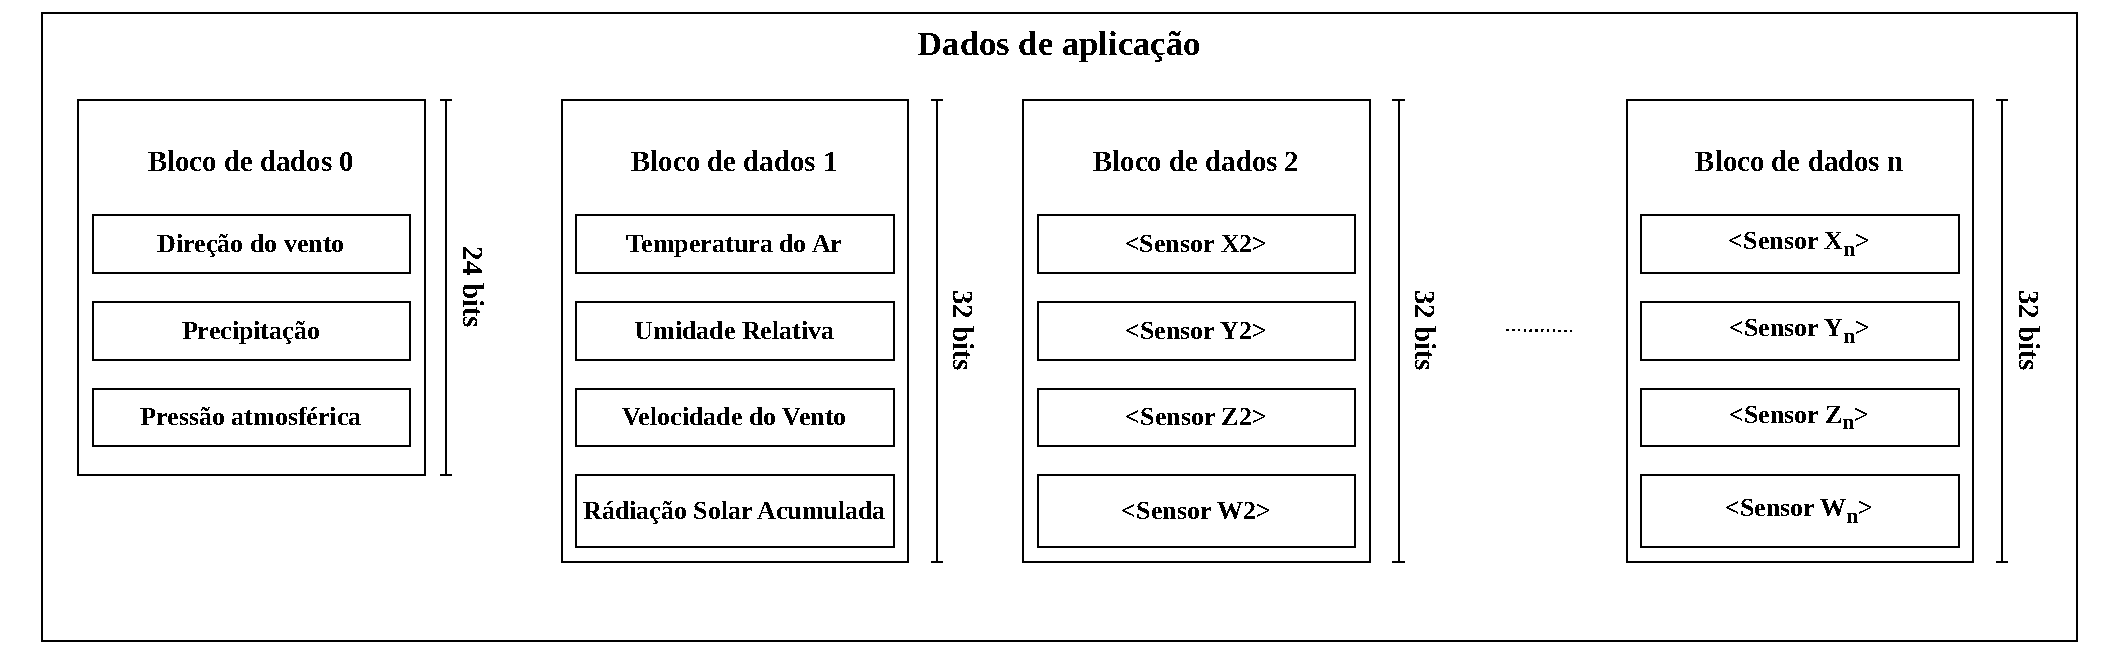
\includegraphics[width=\linewidth]{assets/dados_app.pdf}
\end{figure}


\subsection{Tamanho de mensagem}

O campo de tamanho de mensagem \gls{Tm} é utilizado para informar ao receptor quantos blocos de dados estão sendo transmitidos no datagrama, este campo é formado pelo número de blocos em formato binário \gls{Bm} e pelo bit de pariedade \gls{Pm} para fechar uma seção de 4 bits. Como cada bloco possui 32 bits (exceto o primeiro), é possivel determinar o comprimento total dos dados de aplicação de \gls{Bm} = ($N_b - 1)_{2}$. O número de blocos \gls{Nb}, pode variar de um a oito, resultando no compriemnto esperado de bits no receptor para cada caso, conforme o \autoref{quadro:comprimento-mensagem} abaixo. 

\begin{quadro}[ht]
    \caption{Comprimento em bits para cada tamanho de mensagem ($T_m$)}
    \label{quadro:comprimento-mensagem}
    \small 
    \begin{tabularx}{\textwidth}{>{\centering\arraybackslash}X 
                                  >{\centering\arraybackslash}X 
                                  >{\centering\arraybackslash}X 
                                  >{\centering\arraybackslash}X 
                                  >{\centering\arraybackslash}X}
        \toprule
        \textbf{N° de Blocos} & \textbf{N° de Bits} & \textbf{$B_m$} & \textbf{$P_m$} & \textbf{$T_m$}\\
        \midrule
        1 & 24  & 000 & 0 & 0000\\
        2 & 56  & 001 & 1 & 0011\\
        3 & 88  & 010 & 0 & 0100\\
        4 & 120 & 011 & 1 & 0111\\
        5 & 152 & 100 & 0 & 1000\\
        6 & 184 & 101 & 1 & 1011\\
        7 & 216 & 110 & 0 & 1100\\
        8 & 248 & 111 & 1 & 1111\\
        \bottomrule
    \end{tabularx}
\end{quadro}

Conforme apresentado acima, para cada valor de \gls{Bm}, um valor de \gls{Pm} é calculado. O bit de paridade é calculado de forma a garantir que o número total de bits '1' na mensagem seja par, e é dado por

\vspace{-1em}
\begin{equation}
    P_m = 
    \begin{cases}
    1, & \text{se } \left[ \sum_{i=0}^{B_m} b_i = 0 \right]\mod 2  \\
    0, & \text{se } \left[ \sum_{i=0}^{B_m} b_i = 1 \right]\mod 2 
    \end{cases} \text{.}
\end{equation}

\noindent Ao final, o campo de tamanho de mensagem \gls{Tm} é formado pela concatenação do valor de \gls{Bm} e \gls{Pm}, resultando em um campo de 4 bits \textcite{cnes_services_and_message_formats_ed2_rev2_2006}. 


\subsection{Identificador da PCD}

O identificador da \gls{PCD}, \gls{pcdid}, é um campo de 28 bits presente na estrutura da mensagem do usuário no formato \gls{PTT-A3}. Ele é utilizado para identificar de forma única a \gls{PCD} que está transmitindo a mensagem, sendo essencial para o correto encaminhamento e associação dos dados recebidos no centro de controle do sistema \gls{ARGOS}, \textcite{cnes_services_and_message_formats_ed2_rev2_2006}. 

O \gls{pcdid} é formado por um número de 20 bits, \gls{ipcd}, seguido por oito bits \gls{rpcd} de redundância calculados através da soma (checksum) dos bits do identificador, conforme

\vspace{-1em}
\begin{equation}
R_{PCD} = \left( \sum_{i=0}^{19} I_{PCD} \cdot 2^i \right) \bmod 256 \text{ ,}
\end{equation}
\vspace{-0.2em}
\begin{equation}
    PCD_{ID} = I_{PCD} \oplus R_{PCD} \text{ .}
\end{equation}

\noindent   É importante destacar que a proteção contra erros nesse campo é assegurada de forma indireta pelo uso da codificação convolucional aplicada à mensagem como um todo, além da redundância oferecida pelo número de repetições da mensagem ao longo da passagem do satélite. 


\subsection{Bits de fim de mensagem}

Ao final do datagrama, são inseridos entre sete e nove bits '0' com a finalidade de limpar o registrador do codificador convolucional, dando o encerramento da sequência codificada. A quantidade de bits de fim de mensagem adicionados depende do comprimento total da mensagem do usuário, conforme apresentado na \autoref{quadro:bits-codificacao}. Apesar de não carregar dados úteis a nível de aplicação, esses bits são fundamentais para o correto funcionamento do processo de decodificação \cite{cnes_services_and_message_formats_ed2_rev2_2006}.

\begin{quadro}[ht]
    \caption{Bits adicionados às mensagens do usuário antes da codificação}
    \label{quadro:bits-codificacao}
    \small 
    \begin{tabularx}{\textwidth}{>{\centering\arraybackslash}X 
                                  >{\centering\arraybackslash}X 
                                  >{\centering\arraybackslash}X 
                                  >{\centering\arraybackslash}X}
        \toprule
        \textbf{N° de Blocos} & \textbf{Bits Aplicação} & \textbf{Bits Datagrama} & \textbf{N° bits "0"} \\
        \midrule
        1 &  24 &  56 & 7 \\
        2 &  56 &  88 & 8 \\
        3 &  88 & 120 & 9 \\
        4 & 120 & 152 & 7 \\
        5 & 152 & 184 & 8 \\
        6 & 184 & 216 & 9 \\
        7 & 216 & 248 & 7 \\
        8 & 248 & 280 & 8 \\
        \bottomrule
    \end{tabularx}
    
\end{quadro}


\section{TRANSMISSOR PTT-A3}

Na \autoref{fig:diagrama_blocos_modulador} ilustra-se o diagrama de blocos do transmissor \gls{PTT-A3}. Cada bloco é responsável por uma etapa da transmissão, desde a montagem do datagrama até a modulação em banda passante e a transmissão do sinal \gls{st}.

\begin{figure}[ht]
	\centering
	\caption{Diagrama de blocos do transmissor ARGOS-3}\label{fig:diagrama_blocos_modulador}
	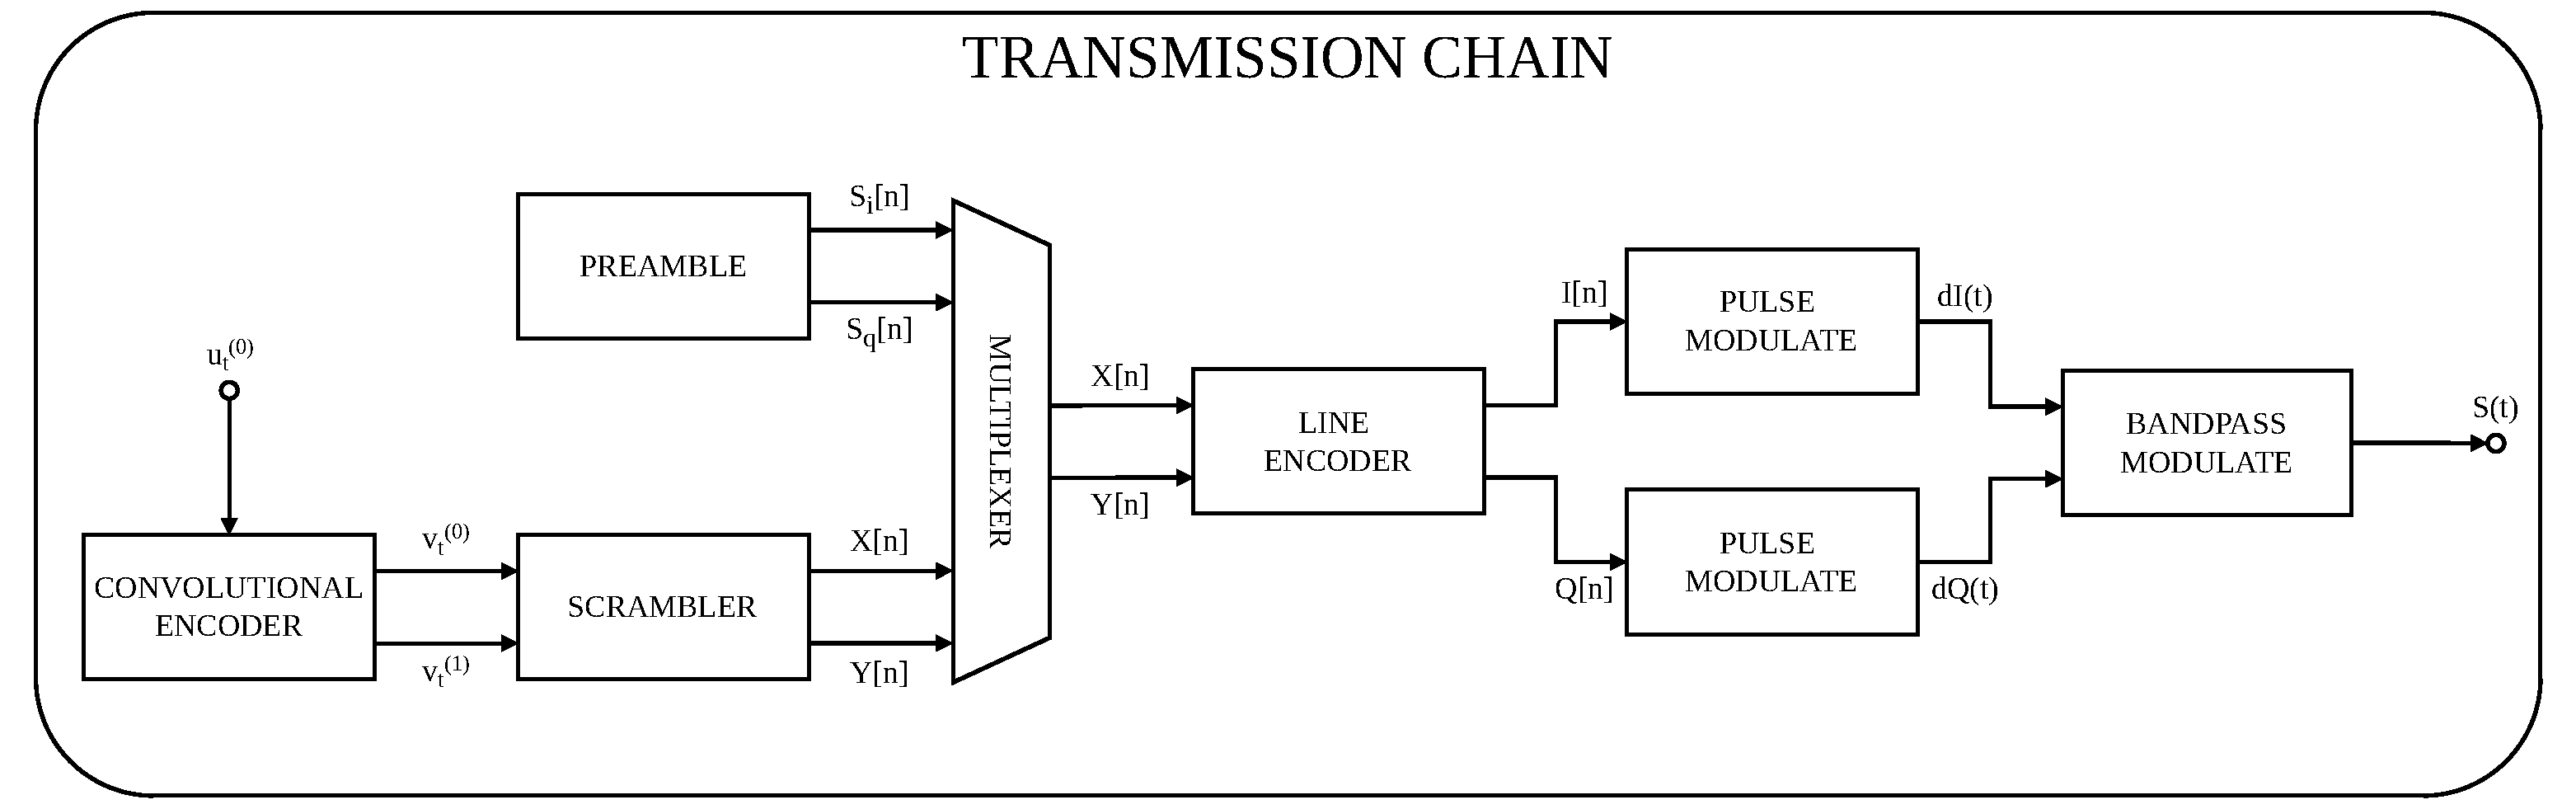
\includegraphics[width=\linewidth]{assets/blocos_modulador.pdf}
    
\end{figure}


\subsection{Codificador convolucional}

Antes da transmissão, os dados do datagrama precisam ser codificados, e esse processo é realizado através de um codificador convolucional. Essa técnica de codificação aplica uma operação lógica sobre uma janela deslizante de bits de entrada \gls{ut}, gerando uma sequência de saída com redundância controlada. Diferente da codificação por bloco, onde os dados são processados em blocos fixos, a codificação convolucional considera a sequência contínua de bits, combinando o bit atual com um número fixo de bits anteriores através de vetores geradores \cite{shu2011error}.

A taxa de codificação utilizada no padrão \gls{PTT-A3} é $R = \text{1/2}$, o que significa que para cada bit de dados de entrada \gls{ut}, são gerados dois bits de saída, um no canal \gls{cI} e outro no canal \gls{cQ}, aumentando a redundância e melhorando a capacidade do sistema de detectar e corrigir erros. Para a codificação convolucional, são utilizados vetores geradores \gls{G0} e \gls{G1}, de acordo com o padrão CCSDS 131.1-G-2 \cite{cnes_services_and_message_formats_ed2_rev2_2006}. A representação binária dos vetores geradores é dada por

\vspace{-1em}
\begin{equation}
    \begin{split}
        G_0 &= 121_{10} \quad \mapsto \quad G_0 = [1, 1, 1, 1, 0, 0, 1] \\
        G_1 &= 091_{10} \quad \mapsto \quad G_1 = [1, 0, 1, 1, 0, 1, 1] \text{.}
    \end{split}
\end{equation}

Os vetores geradores são utilizados para definir a estrutura do registrado do codificação convolucional aplicada à sequência de entrada \gls{ut}, resultando nas saídas \gls{vt0} e \gls{vt1}, que correspondem, respectivamente, aos canais \gls{cI} e \gls{cQ} utilizados posteriormente na modulação \gls{QPSK}. Essa operação pode ser representada por uma multiplicação vetorial entre uma janela deslizante de sete bits da entrada e a matriz formada pelos vetores geradores, conforme

\begin{equation}
\begin{aligned}
    \begin{bmatrix}
        v_t^{(0)} & v_t^{(1)}
    \end{bmatrix}
    &=
    \begin{bmatrix}
        u_{(t)} & u_{(t-1)} & u_{(t-2)} & u_{(t-3)} & u_{(t-4)} & u_{(t-5)} & u_{(t-6)}
    \end{bmatrix} \cdot \\
    &\quad
    \begin{bmatrix}
        1 & 1 & 1 & 1 & 0 & 0 & 1 \\
        1 & 0 & 1 & 1 & 0 & 1 & 1
    \end{bmatrix}^{T}
\end{aligned}
\label{eq:matriz_geradora}
\end{equation}

\noindent que pode ser representada de forma equivalente pelo diagrama de blocos apresentado na \autoref{fig:cod_convolucional} \cite{cnes_services_and_message_formats_ed2_rev2_2006}.

\begin{figure}[ht]
	\centering
	\caption{Diagrama de blocos do codificador convolucional ARGOS-3}
	\label{fig:cod_convolucional}
	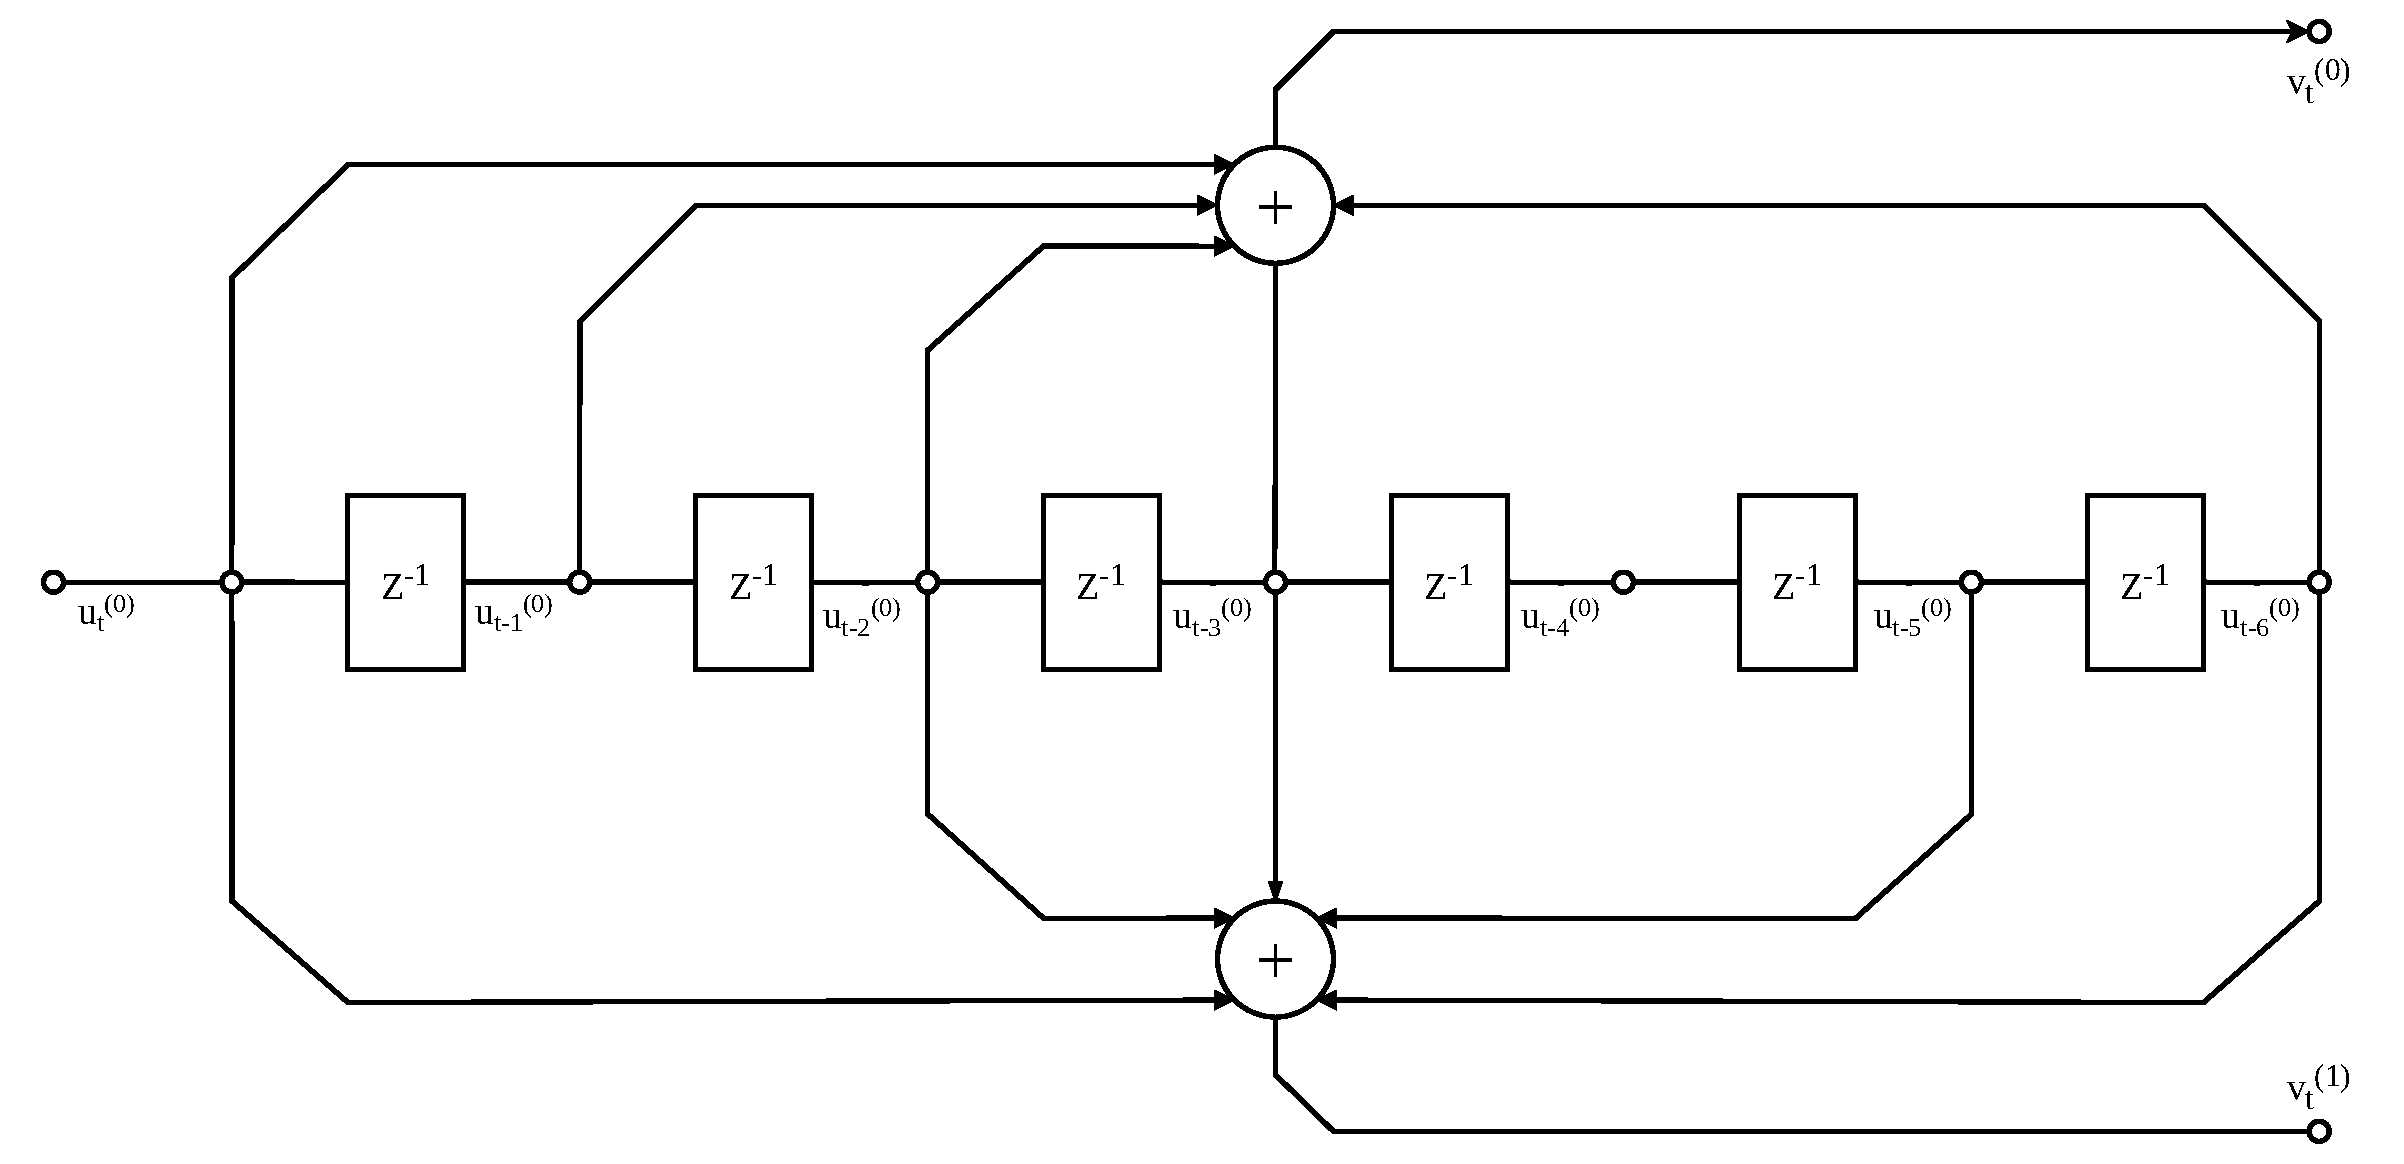
\includegraphics[width=\linewidth]{assets/cod_convolucional.pdf}
\end{figure}


